\chapter{Evaluation}\label{chapter:evaluation}

In this section we provide an extensive experimental evaluation of the HyPer k-Means operator. We compare the different  HyPer implementations to each other as well as to state-of-the-art technologies of clustering data. 
All experiments have been performed on a workstation equipped with sixteen 2.93 GHz CPUs and 64 MB of main memory.


\section{Data Sets}
To provide an objective comparison the execution time per iteration is measured. Therefore the different technologies can be compared fairly and random initialization and internal improvments for faster convergence do not affect the outcome. For the experiments a real world data set is used and four synthetic data sets have been generated. The synthetic data sets represent a high dimensional, a medium size, a medium sized high dimensional and a large size data set as shown in~\autoref{tab:dataset}. All are generated on a uniform random distribution. The data sets are selected in a way that most real world use cases are covered.

\begin{table}[htsb]
  \caption[Data Sets]{Data Sets.}\label{tab:dataset}
  \centering
  \begin{tabular}{l l l l l}
    \toprule
      & Instances & Dimensions & Size (byte) & Size (Gigabyte) \\
    \midrule
      3D Network        & 434874    & 4     & 20673913 & 0.019 \\
      High Dimensional  & 50000     & 50    & 10000000 & 0.009 \\
      Medium Size       & 15M       & 4     & 240000000 & 0.22 \\
      Medium Size HD    & 15M       & 50    & 3000000000 & 2.79 \\
      Large Size        & 150M      & 10    & 6000000000 & 5.59 \\
    \bottomrule
  \end{tabular}
\end{table}



\begin{itemize} 
\item 3D Network: The first data set contains the 3D spatial road network data of a road network in North Jutland, Denmark~\parencite{3dnet}. It is a real world data set available at the UCI Machine Learning Repository~\parencite{uci} and consists of 434874 data points in four dimensions: An id for the road segment, the latitude, the longitude and the altitude of the segment. The id is a large integer, the other dimensions are floating point numbers. The size of the data set is 20,673,913 bytes, therefore it is a rather small data set.

\item High Dimensional: The second dataset is a synthetic data set. It consists of 50000 data points in 50 dimensions. All dimensions are floating point numbers. The size of the data set is 10000000 bytes, hence also a rather small data set, but this time high dimensional.

\item Medium Size: The data set consists of 15 million data points in four dimensions. It is also a synthetic data set generated, all four dimensions containing floating point numbers. The size of the data set is 240000000 bytes and presents the medium size data set in this experiment section.

\item Medium Size HD: The Medium Size HD data set is generated the same way as the Medium Size data set. Instead of four dimensions, this time 50 dimension have been generated. This leads to a growth from 0.22 GB to 2.79 GB.  

\item Large Size: Finally, the large data set consists of 150 million data points in ten dimension. It is also synthetically generated by a random uniform distribution of floating point numbers. The size of the data set is 5.59 GB.
\end{itemize} 



\section{Used Tools}

As already described in chapter \ref{chapter:related}, there exist many tools for data mining. In this chapter we compare a selection of tools implementing the k-Means clustering algorithm with our k-Means HyPer operator. To make the results comparable in a fair manner, we use only tools that give enough information about the clustering process, e.g. number of iterations, total cost and most important, the applied algorithm. Not all tools are implementing the Lloyd algorithm, e.g. the default version of R is the Hartigan-Wong algorithm, an improvement over the standard Lloyed algorithm.
\\
Since k-Means is a non-deterministic algorithm, the number of iterations is another important criteria to make the results comparable. Running time of k-Means depends almost entirely on the number of iterations the algorithm has to make, which depends on the initialization. Therefore the running time should be relative to the number of iterations.
\\
Unfortunately, neither ELKI nor Scipy’s k-Means implementation provide the number of iterations as result. Therefore, a fair comparison is not possible. Weka, R and Julia provide good configuration possibilities as well as a result set that contains information about the number of iterations. Weka is written in Java, while R and Julia are both written in a high level language. Even though, critical code parts are written in C, C++ and Fortran for better performance results, without the overhead of an entire database system behind. Therefore it will be interesting to compare Hyper with the Java written Weka and the optimized R and Julia.
\\
weka, big data?
why not others?
weka arrf format -> loading time, results etc.

\section{Serial Implementation}

In this section we compare the two serial HyPer k-Means implementations: The C++ driven and the LLVM driven approach. For comparison we consider the compilation and the execution time. The compilation time is the time for generating LLVM code, while the execution time is the execution of the k-Means algorithm. Since the compilation time can be seen as a one-time setup time, we expect the execution time to be much larger. 
\\
For each data set, the two HyPer implementations are tested for 3,10 and 20 clusters. For each cluster number the algorithms was executed 100 times with a maximum number of iterations of 10. As result, the median time per iterations in seconds is stated. For better comparability the compilation time is also relative to the number of iterations, even though it does not change for a higher number of iterations.
\\
~\autoref{tab:network_serial} shows the result of the two serial implementations for the network data set. The compilation time is independent of the cluster number $k$ and does not differ among the C++ implementation and the LLVM version. In contrast the execution time increases as the cluster number $k$ increases. This is true for both implementations. For better visualization, ~\autoref{fig:hyper_network} depicts the same result as stacked bar charts.

\begin{table}[htsb]
  \caption[3D Network - Time per Iteration]{3D Network - Time per Iteration.}\label{tab:network_serial}
  \centering
  \begin{tabular}{l l l l l}
    \toprule
      & HyPer C++ & & HyPer LLVM & \\
      k & compilation[s] & execution[s] & compilation[s] & execution[s] \\
    \midrule
      3 & 0.0050 & 0.0680 & 0.0046 & 0.0171 \\
      10 & 0.0044 & 0.0947 & 0.0046 & 0.0502 \\
      20 & 0.0045 & 0.1391 & 0.0046 & 0.0901 \\
    \bottomrule
  \end{tabular}
\end{table}



 While the compilation time is low and constant, the execution time differs among implementation. In particular for $k = 3$, the execution time of the C++ version is almost four times the execution time of the LLVM version. For $k = 10$ it is two times the execution time and for $k = 20$ it is 1.5 times, respectively. On the other hand that means that for a larger cluster number $k$, the LLVM execution time grows  faster than the execution time of the C++ version. Actually, from $k = 3$ to $k = 10$, the LLVM version grows by a factor of 2.9, while the C++ grows by 1.4. From $k = 3$ to $k = 20$ the growth is even more significant, from factor 2 for the C++ version to 5.3 for the LLVM version.


\begin{figure}[htsb]
  \centering
  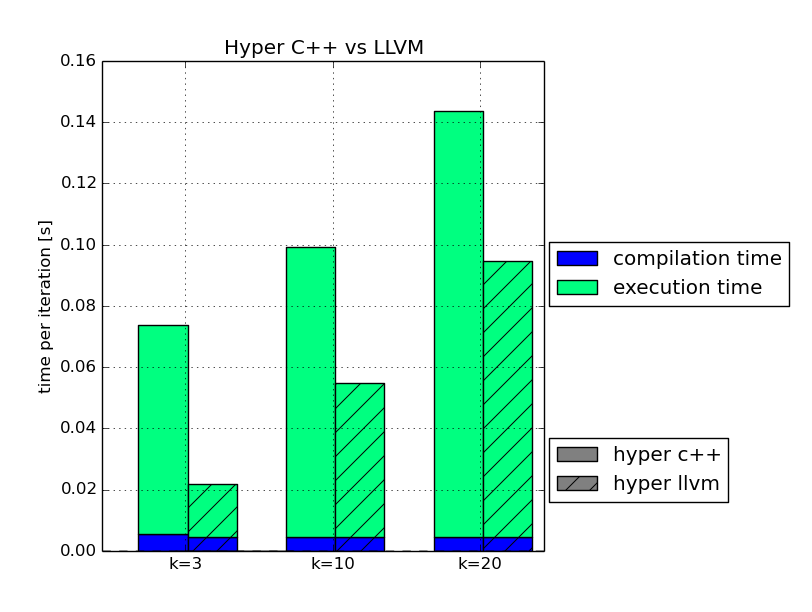
\includegraphics[scale=0.4, trim="0cm 1.5cm 0cm 0cm"]{figures/charts/hyper_network}
  \caption[3D Network - Time per Iteration]{3D Network - Time per Iteration.}
  \label{fig:hyper_network}
\end{figure}

This gives us the first interesting results. Although the C++ version is implementing k-Means using LLVM only for generated functions, the compilation time does not differ to the LLVM version, where not only the functions but also the entire algorithm is written in LLVM. Nevertheless, the functions for computing the distance and updating the centers are generated in LLVM for both implementations which is an explanation for the similar compilation times. In C++ these functions are generated as functions callable from C++, while in the LLVM version, the code is directly embedded into an LLVM program structure. The difference between the two seems to be insignificant.
\\
Regarding the execution time, the LLVM version is much faster than the C++ version. One reason is that the C++ implementation has many function calls between the \texttt{compile time} and the \texttt{runtime system}. For the LLVM system these calls are not necessary and the data remains in the CPU registers. The second advantage is that the entire algorithm is compiled in LLVM code resulting in a very efficient code, optimized on a lower level than even possible with C++ code.


\begin{table}[htsb]
  \caption[High Dimensional - Time per Iteration]{High Dimensional - Time per Iteration.}\label{tab:hd_serial}
  \centering
  \begin{tabular}{l l l l l}
    \toprule
      & HyPer C++ & & HyPer LLVM & \\
      k & compilation[s] & execution[s] & compilation[s] & execution[s] \\
    \midrule
      3  & 0.1278 & 0.0522 & 0.0933 & 0.0327 \\
      10 & 0.1287 & 0.1171 & 0.0933 & 0.0706 \\
      20 & 0.1299 & 0.2070 & 0.0933 & 0.1252 \\
    \bottomrule
  \end{tabular}
\end{table}

~\autoref{tab:hd_serial} shows the result of the same experiment with the high dimensional data set. In contrary to the network data set the compilation time is slightly different between the C++ and the LLVM implementation. Furthermore for both versions the compilation time is larger than the execution time for $k = 3$ and almost equal for $k = 10$. Only for $k = 20$ the execution time is larger than the compilation time, as depicted in~\autoref{fig:hyper_50000}.

\begin{figure}[htsb]
  \centering
  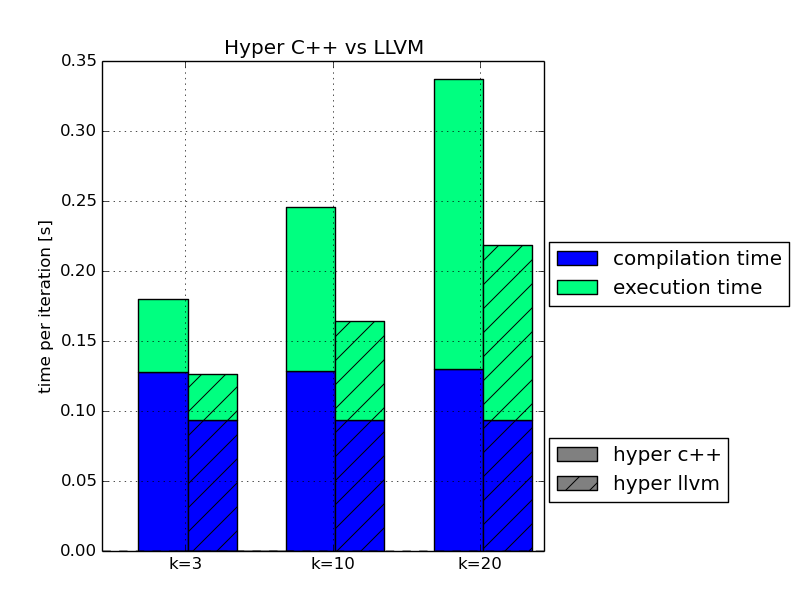
\includegraphics[scale=0.4, trim="0cm 1.5cm 0cm 0cm"]{figures/charts/hyper_50000}
  \caption[High Dimensional - Time per Iteration]{High Dimensional - Time per Iteration.}
  \label{fig:hyper_50000}
\end{figure}

Again, the compilation time stays constant for different values of $k$. The increase of compilation time is induced by the high dimensionality: For each dimension additional code has to be generated. Therefore a data set with four dimension is faster to compile than a data set with 50 dimensions. 
The difference in the running time is similar to the network data set even though the increase in performance is not as significant. For $k = 3$, LLVM is faster by a factor 1.6 and for $k = 10$ and $k = 20$ by facor 1.7. This time the increase in execution time is strongly correlated. From $k = 3$ to $k = 10$, the LLVM version and the C++ version grow by a factor of 2.2. From $k = 3$ to $k = 10$, the LLVM version grows by a factor of 4, while the C++ grows by 3.8.
\\
Interestingly, ten iterations terminate much quicker for the network data set than for the high dimensional data set, even though the network set is 2.1 times as large as the high dimensional data set. Even if we omit the compilation time which stays constant for a growing number of iterations, the execution time of the network data set is only for the C++ implemenation and $k = 3$ slower than the high dimensional data set. That shows us that our implementation performs much better for low dimensional data sets.
\\
\\
~\autoref{tab:med_serial} and ~\autoref{tab:med_hd_serial} show the same experiment for larger data sets. Both consist of 15 million instances, the first of four dimensions and the second of 50 dimensions. The compilation time of the medium size data set is similar to the network data set since both consist of four dimensions. The same is true for the medium size high dimensional data set and the smaller high dimensional data set. This proves that the compilation time is independent on the data size and only affect by the number of dimensions. However, as the number of instances is growing, the compilation time is not a significant factor for the overall execution time, as~\autoref{fig:hyper_15Mxhd} shows: The compilation time is not even visible plotting the data as barcharts as before.

\begin{table}[htsb]
  \caption[Medium Size - Time per Iteration]{Medium Size - Time per Iteration.}
  \label{tab:med_serial}
  \centering
  \begin{tabular}{l l l l l}
    \toprule
      & HyPer C++ & & HyPer LLVM & \\
      k & compilation[s] & execution[s] & compilation[s] & execution[s] \\
    \midrule
      3  & 0.0041 & 2.3779 & 0.0047 & 0.9191 \\
      10 & 0.0041 & 3.2856 & 0.0047 & 2.1001 \\
      20 & 0.0041 & 4.6765 & 0.0047 & 3.4518 \\
    \bottomrule
  \end{tabular}
\end{table}


\begin{table}[htsb]
  \caption[Medium Size High Dimensional - Time per Iteration]{Medium Size High Dimensional - Time per Iteration.}
  \label{tab:med_hd_serial}
  \centering
  \begin{tabular}{l l l l l}
    \toprule
      & HyPer C++ & & HyPer LLVM & \\
      k & compilation[s] & execution[s] & compilation[s] & execution[s] \\
    \midrule
      3  & 0.1127 & 16.2787 & 0.0935 & 10.3302 \\
      10 & 0.1127 & 34.0051 & 0.0935 & 22.0209 \\
      20 & 0.1126 & 59.2904 & 0.0935 & 38.7046 \\
    \bottomrule
  \end{tabular}
\end{table}

Obviously the execution time for the high dimensional data set is much larger again. For the C++ implementation the execution time is increased by a factor of 6.8 for $k = 3$, 10.3 for $k = 10$ and 12.6 for $k = 20$. For the LLVM implementation it is 11.2, 10.5, 11.2, respectively. Since the high dimensional data set is actually larger by a factor of 12.7, the values are strongly correlated to the growth of the data set.

\begin{figure}[htsb]
  \centering
  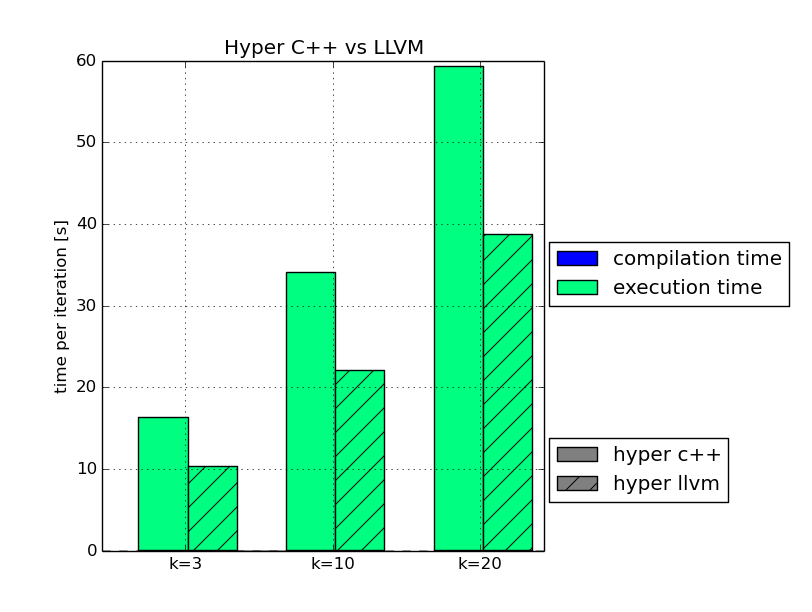
\includegraphics[scale=0.4, trim="0cm 1.5cm 0cm 0cm"]{figures/charts/hyper_15Mxhd}
  \caption[Medium Size High Dimensional - Time per Iteration]{Medium Size High Dimensional - Time per Iteration.}
  \label{fig:hyper_15Mxhd}
\end{figure}




~\autoref{tab:large_serial} shows the same experiment for the large data set. The data set consists of ten dimensions and therefore the compilation time increases compared to the data sets with four dimensions by a factor of around 2. Since the data set has a size of 5.59 GB the difference in the execution time is very significant. Again, the LLVM implementation is faster by around 20 seconds independent of the cluster number $k$.



\begin{table}[htsb]
  \caption[Large Size - Time per Iteration]{Large Size - Time per Iteration.}
  \label{tab:large_serial}
  \centering
  \begin{tabular}{l l l l l}
    \toprule
      & HyPer C++ & & HyPer LLVM & \\
      k & compilation[s] & execution[s] & compilation[s] & execution[s] \\
    \midrule
      3  & 0.0088 & 37.2804 & 0.0097 & 18.3734 \\
      10 & 0.0088 & 62.0034 & 0.0097 & 40.4783 \\
      20 & 0.0191 & 92.5868 & 0.0097 & 67.2364 \\
    \bottomrule
  \end{tabular}
\end{table}


In conclusion the compilation time is not affected if the number of instances gets large but only if the number of dimensions grows. The compilation time is similar between the LLVM version and the C++ version. Usually, the execution time outnumbers the compilation time by several factors. The only exception is the small, high dimensional data set as shown in the experiment. Here, the compilation time can be slower than the execution time.
\\
Furthermore the execution time grows by number of instances and is much faster for the LLVM implementation. With equality regarding the compilation and a performance decrease in execution time the LLVM version was for all experiments the best choice regarding the running time of the k-Means algorithm.


\section{Performance Test}

In this section we compare our serial HyPer implementations to Weka, R and Julia’s implementation of the k-Means algorithm. As algorithm, the Lloyd algorithm with a maximum iteration number of ten is chosen. Apart from the large data set, the algorithm is executed 100 times for $k = 3, 10$ and $20$, respectively. For the large data set, the algorithm is executed ten times. The result is then presented as the execution time per iteration. For each algorithm the median, the 90th percentile and the 95th percentile are given for every $k$. 
\\
\begin{table}[htsb]
  \caption[3D Network - Time per Iteration]{3D Network - Time per Iteration.}
  \label{tab:network_all}
  \centering
  \begin{tabular}{l l l l l l l l l l l l l}
    \toprule
      & \multicolumn{3}{c}{Julia} & \multicolumn{3}{c}{R} & \multicolumn{3}{c}{HyPer C++} & \multicolumn{3}{c}{HyPer LLVM}  \\
      k & 3 & 10 & 20 & 3 & 10 & 20 & 3 & 10 & 20 & 3 & 10 & 20 \\
    \midrule
      50  & 0.21 & 0.22 & 0.29 & 0.03 & 0.04 & 0.08 & 0.08 & 0.10 & 0.14 & 0.02 & 0.06 & 0.10 \\
      50  & 0.27 & 0.30 & 0.32 & 0.06 & 0.06 & 0.09 & 0.08 & 0.10 & 0.14 & 0.02 & 0.06 & 0.10 \\
      50  & 0.31 & 0.35 & 0.35 & 0.08 & 0.07 & 0.10 & 0.08 & 0.10 & 0.14 & 0.02 & 0.06 & nnnn \\
    \bottomrule
  \end{tabular}
\end{table}

\begin{figure}[htsb]
  \raggedleft
  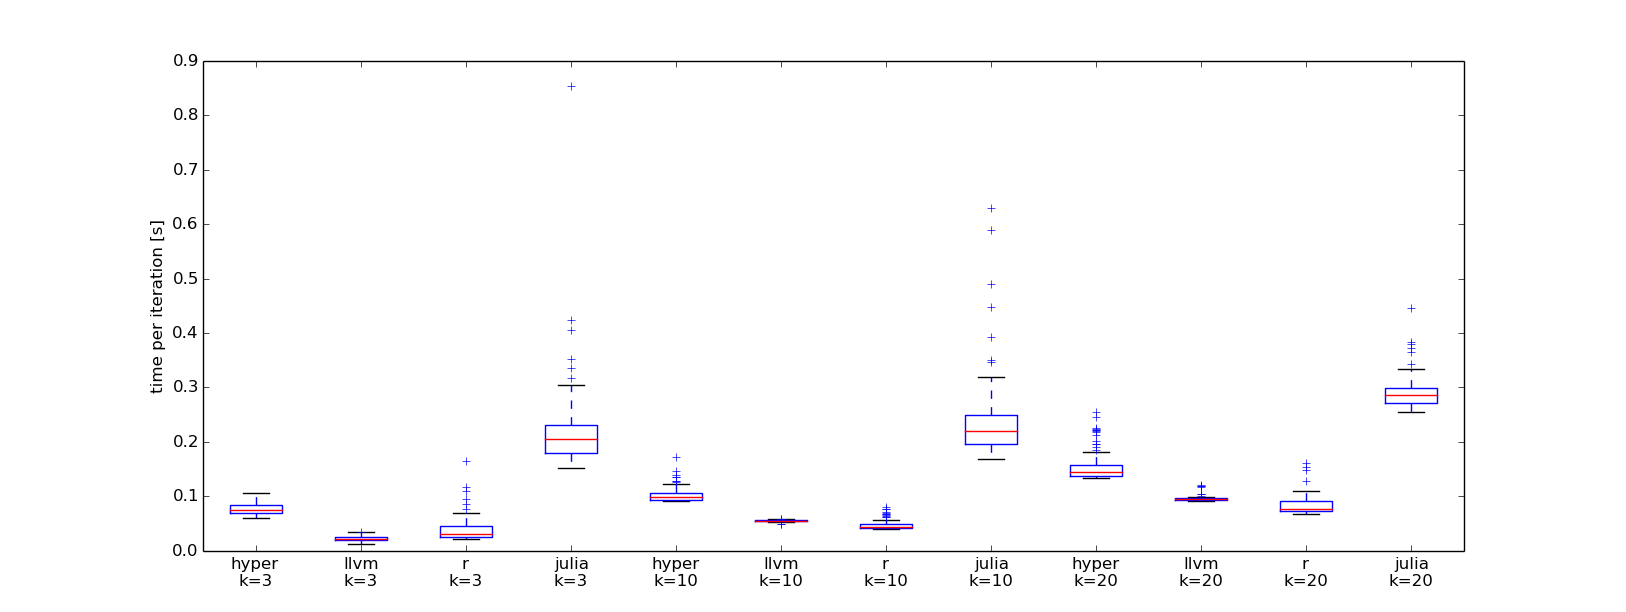
\includegraphics[scale=0.4, trim="0cm 1cm 0cm 0cm"]{figures/charts/network_all}
  \caption[3D Network - Time per Iteration]{3D Network - Time per Iteration.}
  \label{fig:network_all}
\end{figure}

The result of the network data set is presented in Table: network. The median, the 90th and 95th percentile are listed to show the variance of the data. As we already know, the HyPer LLVM implementation outnumbers  the C++ version. Julia is the slowest, while R competes quite well with the LLVM version and is even faster for k equals 10 and 20. Figure 1 shows the results as a boxplot.
However, all tested programs differ in time per iterations in a few hundred milliseconds, therefore the differences are not very significant.
\\
Running the same experiment on the high dimensional data set we see a different result. As Table 2 shows, both HyPer C++ and the LLVM version are slower compared to the network data set, while R is almost the same. Interestingly, julia’s k-Means is now as fast as the R implementation, for k = 10 and 20 it is even faster. Figure xx shows this results as a boxplot. 
\\
This result gives us interesting knowledge about the implementation. An increase in dimensions and decrease in instances does not affect R significantly. On the other hand, julia shows much better results as dimensions increases and seems to be optimized for high dimensions. Both HyPer implementations cannot compete with R and julia regarding the running time. As we already observed comparing the two implementations in greater detail in section 7.2x, the compilation time of the two operators is quite high when using high dimensional data.
\\
For comparison, Figure x shows the same boxplot of the high dimensional data, but this time omitting the compilation time for the two HyPer implementations. This time, for k=3, the LLVM version is the fastest, while with growing k R and julia are faster, but not that significantly anymore. The C++ version remains the slowest. However, this result shows that the code generation for high dimensional data sets with less instances is not optimal and can be a ?ansatz? for future optimization.
\\
Next, we discuss the performance on medium and large size data sets with four and ten dimensions, respectively. This time, the compilation time should not be a limiting factor. Table M and Figure M show the results for  the medium size data set. This time, julia performs the worst followed by the C++ implementation. LLVM and R are quite close, even though for growing k R outperforms the LLVM version. 
\\
Regarding the large data set, the order changed. Julia and the HyPer’s C++ version are still slow, while the LLVM version outperforms the R version as Table L and Figure L show.
\\
In conclusion, the experiments show that HyPer’s k-Means operator can compete with existing tools for clustering. Rearding the LLVM implementation, HyPer and R show the best results. Only for the high dimensional data set, julia shows the best results. If we take into account that the k-Means algorithm runs on top of an entire database with all its overhead, these result are very affirmative for future improvements and the implementations of other operators on HyPer.


\begin{table}[htsb]
  \caption[High Dimensional - Time per Iteration]{High Dimensional - Time per Iteration.}
  \label{tab:highdim_all}
  \centering
  \begin{tabular}{l l l l l l l l l l l l l}
    \toprule
      & \multicolumn{3}{c}{Julia} & \multicolumn{3}{c}{R} & \multicolumn{3}{c}{HyPer C++} & \multicolumn{3}{c}{HyPer LLVM}  \\
      k & 3 & 10 & 20 & 3 & 10 & 20 & 3 & 10 & 20 & 3 & 10 & 20 \\
    \midrule
      50  & 0.04 & 0.05 & 0.07 & 0.03 & 0.05 & 0.08 & 0.18 & 0.24 & 0.35 & 0.13 & 0.16 & 0.22 \\
      50  & 0.04 & 0.05 & 0.07 & 0.04 & 0.06 & 0.10 & 0.21 & 0.34 & 0.40 & 0.13 & 0.16 & 0.22 \\
      50  & 0.04 & 0.05 & 0.07 & 0.05 & 0.07 & 0.11 & 0.22 & 0.35 & 0.44 & 0.13 & 0.17 & 0.22 \\
    \bottomrule
  \end{tabular}
\end{table}

Verhaeltnis: um wie viel schlechter wirds im vergleich zum network set?
verhaeltnis zu einander
verhaeltnis zu den ks



\begin{table}[htsb]
  \caption[Medium Size - Time per Iteration]{Medium Size - Time per Iteration.}
  \label{tab:medium_all}
  \centering
  \begin{tabular}{l l l l l l l l l l l l l}
    \toprule
      & \multicolumn{3}{c}{Julia} & \multicolumn{3}{c}{R} & \multicolumn{3}{c}{HyPer C++} & \multicolumn{3}{c}{HyPer LLVM}  \\
      k & 3 & 10 & 20 & 3 & 10 & 20 & 3 & 10 & 20 & 3 & 10 & 20 \\
    \midrule
      50  & 5.42 & 7.61 & 10.62 & 0.77 & 1.61 & 2.50 & 2.38 & 3.29 & 4.68 & 0.92 & 2.10 & 3.46 \\
      50  & 5.43 & 7.65 & 10.71 & 0.79 & 1.63 & 2.55 & 2.57 & 3.44 & 4.77 & 0.94 & 2.14 & 3.51 \\
      50  & 5.44 & 7.70 & 10.91 & 0.80 & 1.63 & 2.56 & 2.64 & 3.45 & 4.84 & 0.94 & 2.14 & 3.52 \\
    \bottomrule
  \end{tabular}
\end{table}



\begin{table}[htsb]
  \caption[Medium Size HD - Time per Iteration]{Medium Size HD - Time per Iteration.}
  \label{tab:medium_hd_all}
  \centering
  \begin{tabular}{l l l l l l l l l l l l l}
    \toprule
      & \multicolumn{3}{c}{Julia} & \multicolumn{3}{c}{R} & \multicolumn{3}{c}{HyPer C++} & \multicolumn{3}{c}{HyPer LLVM}  \\
      k & 3 & 10 & 20 & 3 & 10 & 20 & 3 & 10 & 20 & 3 & 10 & 20 \\
    \midrule
      50  & 11.46 & 15.69 & 21.67 & 9.43 & 15.48 & 23.77 & 16.39 & 34.12 & 59.40 & 10.42 & 22.11 & 38.80 \\
      50  & 11.51 & 15.81 & 21.69 & 9.50 & 15.50 & 23.79 & 16.77 & 36.11 & 59.53 & 10.44 & 22.12 & 38.84 \\
      50  & 11.65 & 15.83 & 21.70 & 9.64 & 15.58 & 23.79 & 17.29 & 42.15 & 59.57 & 10.45 & 22.13 & 38.84 \\
    \bottomrule
  \end{tabular}
\end{table}



\begin{table}[htsb]
  \caption[Large Size - Time per Iteration]{Large Size - Time per Iteration.}
  \label{tab:network_all}
  \centering
  \begin{tabular}{l l l l l l l l l l l l l}
    \toprule
      & \multicolumn{3}{c}{Julia} & \multicolumn{3}{c}{R} & \multicolumn{3}{c}{HyPer C++} & \multicolumn{3}{c}{HyPer LLVM}  \\
      k & 3 & 10 & 20 & 3 & 10 & 20 & 3 & 10 & 20 & 3 & 10 & 20 \\
    \midrule
      50  & 65.62 & 90.37 & 132.39 & 29.47 & 48.21 & 72.40 & 37.29 & 62.01 & 92.60 & 18.38 & 40.49 & 67.25 \\
      50  & 65.72 & 92.01 & 135.87 & 30.80 & 54.73 & 77.27 & 37.50 & 62.41 & 92.86 & 18.44 & 40.72 & 67.57 \\
      50  & 65.78 & 92.27 & 137.21 & 33.08 & 55.02 & 77.97 & 37.52 & 62.72 & 92.95 & 18.46 & 40.72 & 67.63 \\
    \bottomrule
  \end{tabular}
\end{table}




\begin{figure}[htsb]
  \raggedleft
  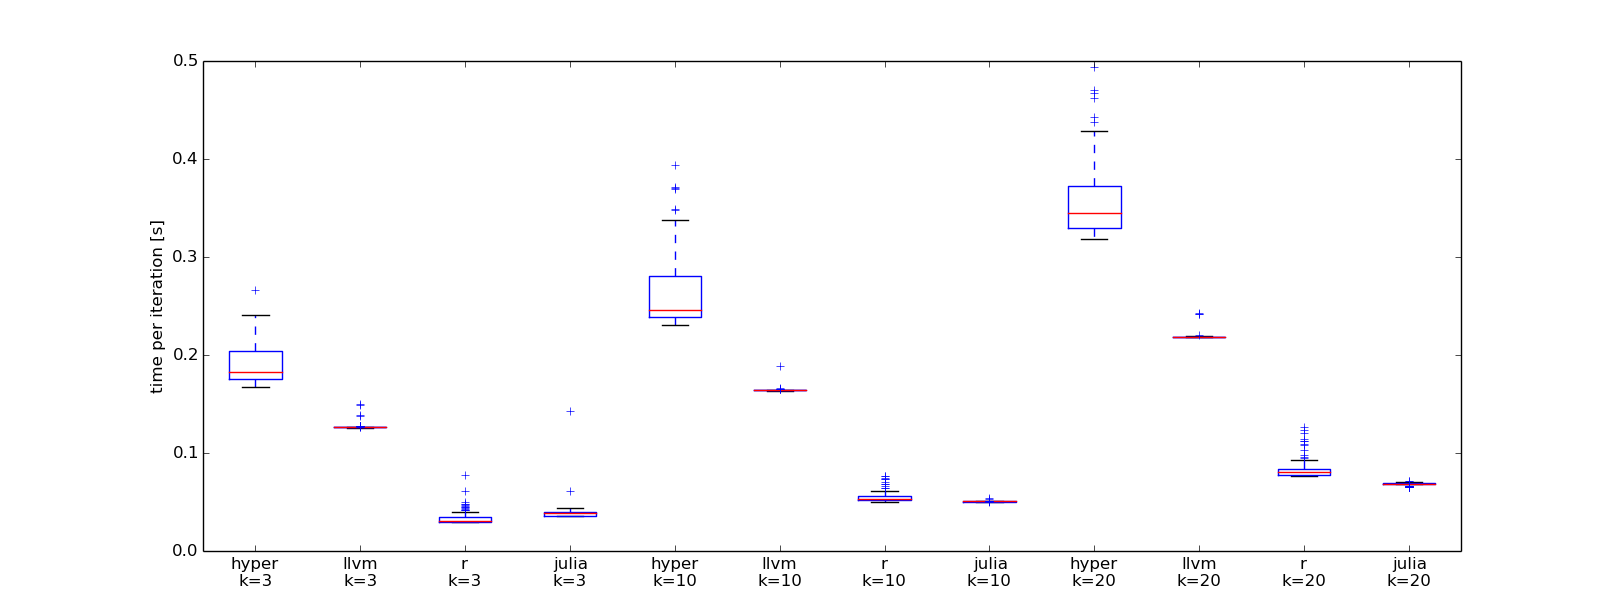
\includegraphics[scale=0.4, trim="0cm 1cm 0cm 0cm"]{figures/charts/50000_all}
  \caption[High Dimensional - Time per Iteration]{High Dimensional - Time per Iteration.}
  \label{fig:50000_all}
\end{figure}

\begin{figure}[htsb]
  \raggedleft
  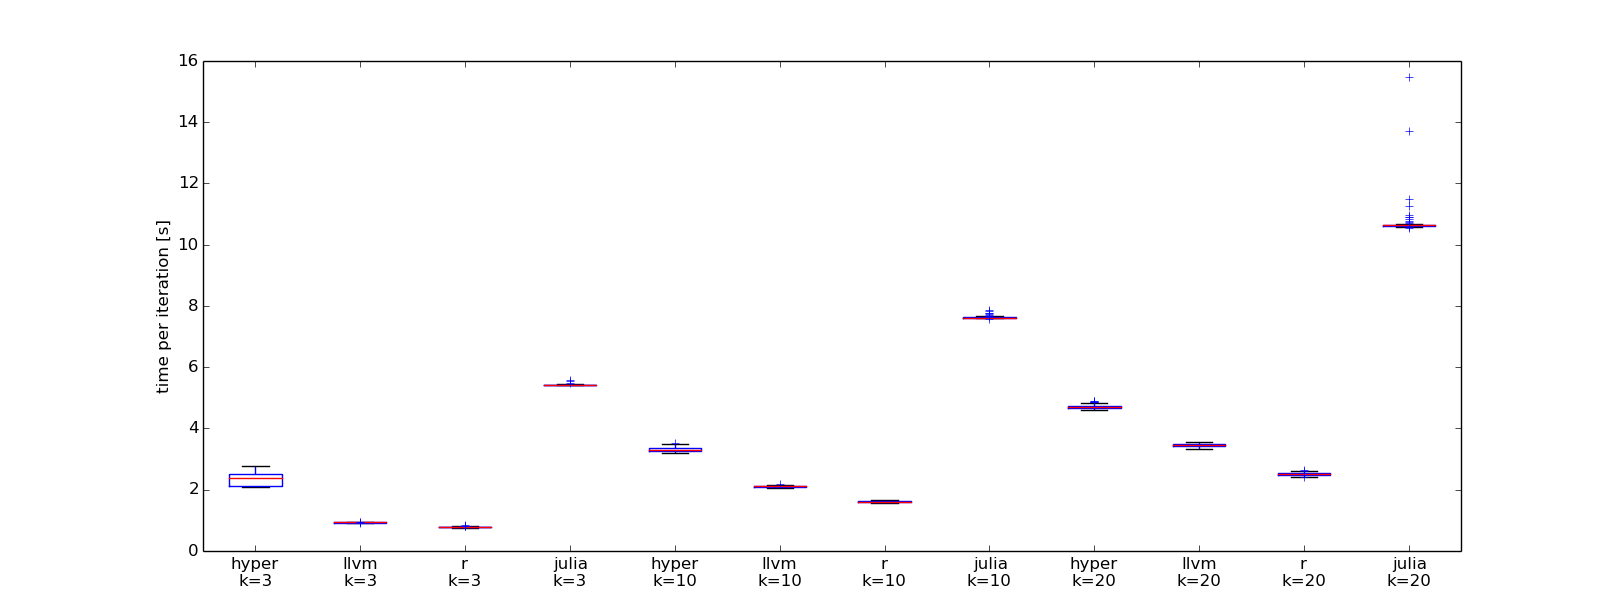
\includegraphics[scale=0.4, trim="0cm 1cm 0cm 0cm"]{figures/charts/15M_all}
  \caption[Medium Size - Time per Iteration]{Medium Size - Time per Iteration.}
  \label{fig:15M_all}
\end{figure}


\begin{figure}[htsb]
  \raggedleft
  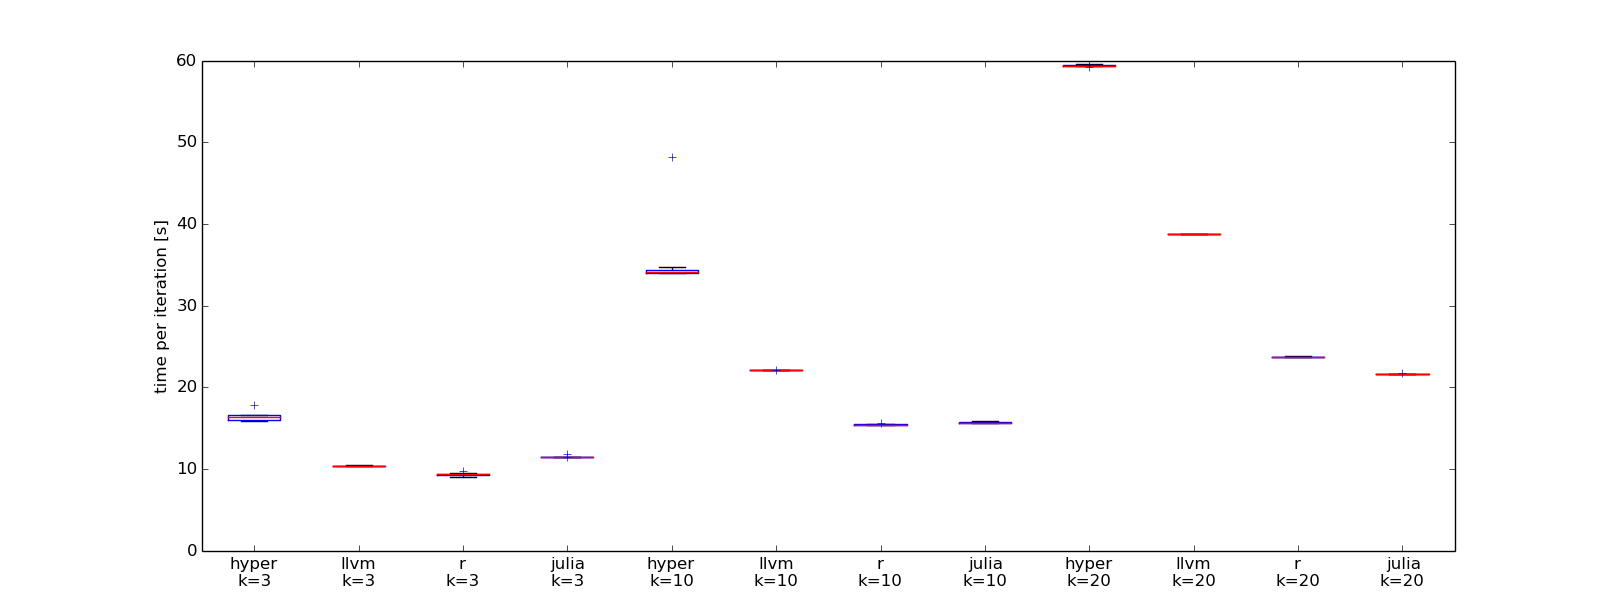
\includegraphics[scale=0.4, trim="0cm 1cm 0cm 0cm"]{figures/charts/15Mxhd_all}
  \caption[Medium Size HD - Time per Iteration]{Medium Size HD - Time per Iteration.}
  \label{fig:15Mxhd_all}
\end{figure}


\begin{figure}[htsb]
  \raggedleft
  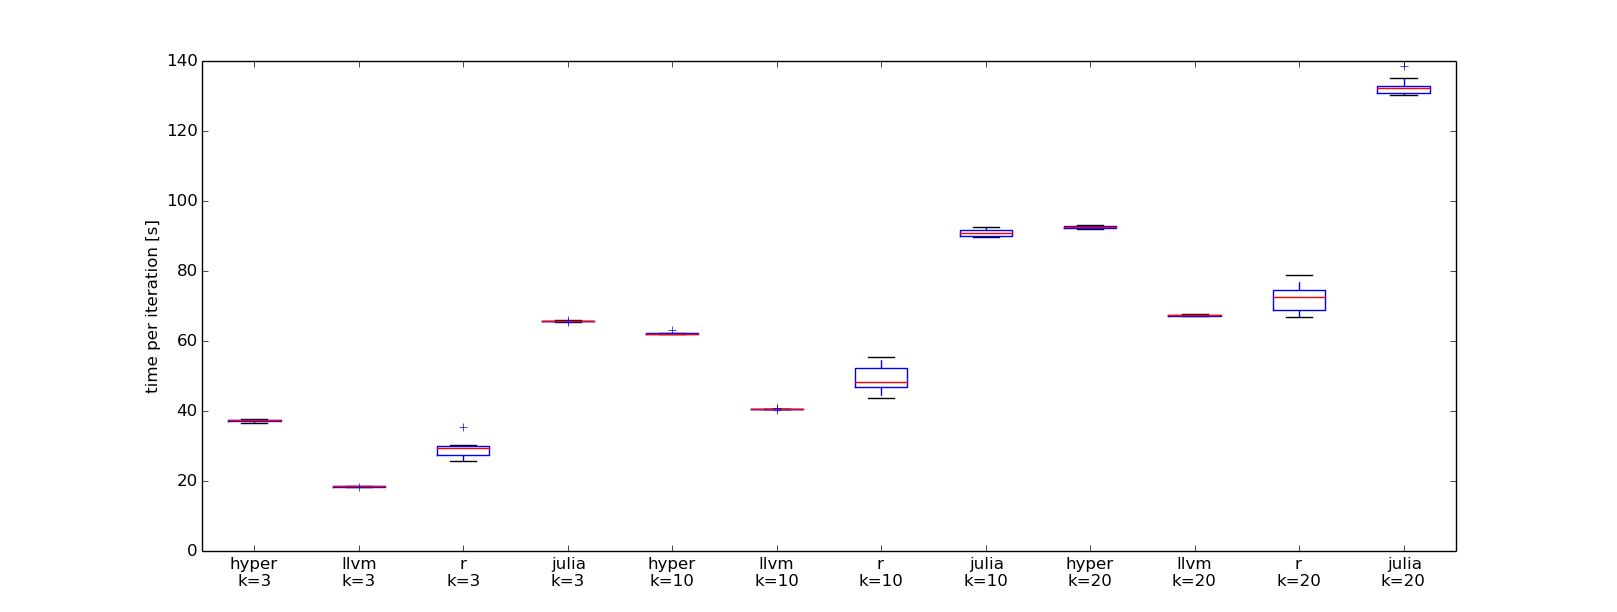
\includegraphics[scale=0.4, trim="0cm 1cm 0cm 0cm"]{figures/charts/150M_all}
  \caption[Large Size - Time per Iteration]{Large Size - Time per Iteration.}
  \label{fig:150M_all}
\end{figure}



\section{Parallel Implementation}


So far we compared the serial execution of the HyPer k-Means operator with julia and R. In 7.4 we figured out that the LLVM implementation outperforms the C++ version on all data sets we tested on. In 7.5 we compared the performance against julia and R and showed that HyPer is able to compete with the existing solutions.
\\
However, as data sets grow serial execution takes more and more time, making real-time data mining almost impossible. To improve performance, HyPer operators benefit from multi-threaded execution. In this section we compare the parallel implementation of the HyPer kMeans operator with the LLVM version and the R implementation. For comparison, we use the medium and the large data set.
\\
Table x depicts the time per iteration for k =3, 10 and 20. As before, the medium, the 90th and 95th percentile of 100 iterations on a 16 core machine are presented. For k equals 3, we see that both the R and the LLVM version are faster than the parallel version. However, with growing k, the parallel version outperforms R and the LLVM version. This is also shown in the bar chart in Figure xx.

\begin{table}[htsb]
  \caption[3D Network - Time per Iteration]{3D Network - Time per Iteration.}
  \label{tab:network_all}
  \centering
  \begin{tabular}{l l l l l l l l l l }
    \toprule
      & \multicolumn{3}{c}{R} & \multicolumn{3}{c}{HyPer C++} & \multicolumn{3}{c}{HyPer LLVM}  \\
      k & 3 & 10 & 20 & 3 & 10 & 20 & 3 & 10 & 20 \\
    \midrule
      50  & 0.03 & 0.04 & 0.08 & 0.08 & 0.10 & 0.14 & 0.02 & 0.06 & 0.10 \\
      90  & 0.06 & 0.06 & 0.09 & 0.08 & 0.10 & 0.14 & 0.02 & 0.06 & 0.10 \\
      95  & 0.08 & 0.07 & 0.10 & 0.08 & 0.10 & 0.14 & 0.02 & 0.06 & nnnn \\
    \bottomrule
  \end{tabular}
\end{table}


The reason for performing better than R and LLVM for growing k is the the running time of the parallel execution is almost independent of k. While R and the LLVM version grow by seconds as k grows, the parallel version grows insignificantly by around 200 milliseconds. 
\\
Unfortunately, for the medium size data set and small k, the parallel version cannot compete with the LLVM and R algorithm.  First, we have to take into account the overhead of the parallel process. Second, we are using the slower C++ version of the HyPer kMeans operator. Even though parts of it are parallelized, we still have all the downsides of many function calls between the runtime and the compile time system and of the high-level C++ constructs.

\begin{figure}[htsb]
  \centering
  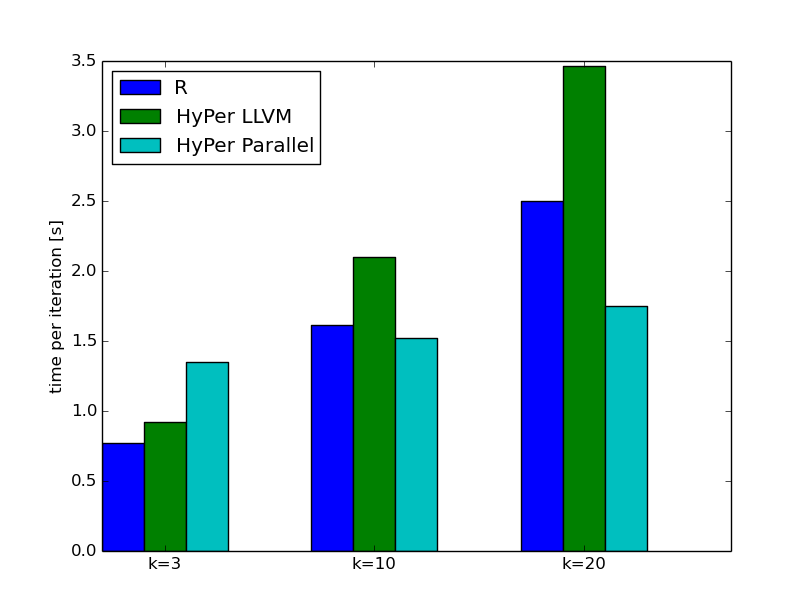
\includegraphics[scale=0.4, trim="0cm 1.5cm 0cm 0cm"]{figures/charts/final_15M}
  \caption[Medium Size - Time per Iteration]{Medium Size - Time per Iteration.}
  \label{fig:final_15M}
\end{figure}

Table x shows the same experiment on the large size data set. The table shows the median, the 90th and the 95th percentile. For better visualization, the bar chart in Figure x depicts the median value of the R, LLVM and parallel execution. 

\begin{table}[htsb]
  \caption[3D Network - Time per Iteration]{3D Network - Time per Iteration.}
  \label{tab:network_all}
  \centering
  \begin{tabular}{l l l l l l l l l l }
    \toprule
      & \multicolumn{3}{c}{R} & \multicolumn{3}{c}{HyPer C++} & \multicolumn{3}{c}{HyPer LLVM}  \\
      k & 3 & 10 & 20 & 3 & 10 & 20 & 3 & 10 & 20 \\
    \midrule
      50  & 0.03 & 0.04 & 0.08 & 0.08 & 0.10 & 0.14 & 0.02 & 0.06 & 0.10 \\
      90  & 0.06 & 0.06 & 0.09 & 0.08 & 0.10 & 0.14 & 0.02 & 0.06 & 0.10 \\
      95  & 0.08 & 0.07 & 0.10 & 0.08 & 0.10 & 0.14 & 0.02 & 0.06 & nnnn \\
    \bottomrule
  \end{tabular}
\end{table}


This time, however, the parallel version outperforms the R and LLVM version for all k’s. Thus, the performance difference gets remarkably as k grows. We experience the same effect as for the medium size data set: A change in k affects only slightly the performance of the parallel version, while it decreases the performance of the serial implementations. 
\\
In the following paragraphs we look at the parallel execution in greater detail. 


\begin{figure}[htsb]
  \centering
  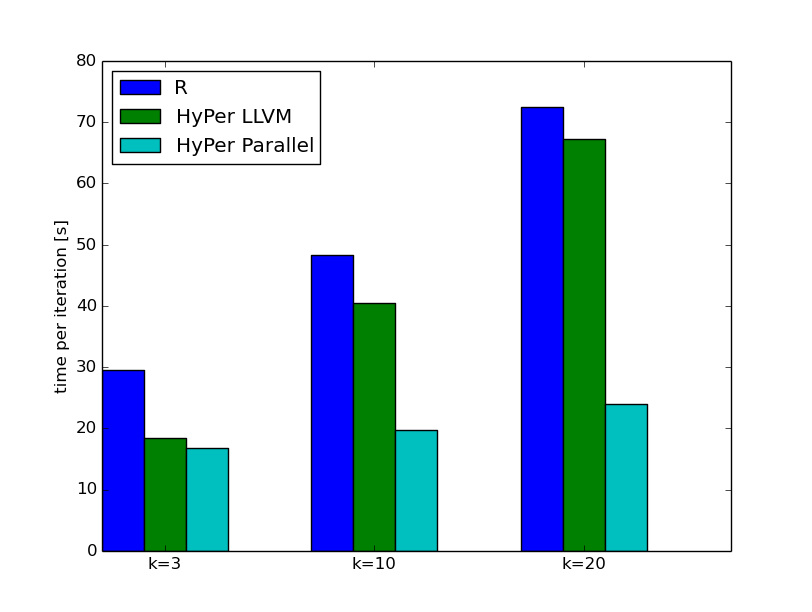
\includegraphics[scale=0.4, trim="0cm 1.5cm 0cm 0cm"]{figures/charts/final_150M}
  \caption[Large Size - Time per Iteration]{Large Size - Time per Iteration.}
  \label{fig:final_150M}
\end{figure}


